
\section{Proofs} \label{app:proofs}

\subsection{Proofs from Section~\ref{sec:equi-and-dual}}
	\noindent\textbf{Proof of Lemma~\ref{lemma:U-convex-compact}}
	First, we state a lemma due to \citet[Theorems 1 and 4]{dvoretzky1951relations}. Here, we assume that there is an underlying $\sigma$-algebra $\mathcal{M}$ on $\Theta$ corresponding to all measures $\mu_i$.
	\begin{lemma}
		Let $\mu_i$ be finite measures on $\Theta$, $i\in m$. 
		Let 
		\begin{align*}
			& \mathcal{X} = \left\{ (x_1, \dots, x_p): \sum_j x_j = \ones, \, \almeve,\, \text{each $x_j$ is a nonnegative measurable function on $\Theta$} \right\}, \\
			& \mathcal{S} = \left\{ (\Theta_1, \dots, \Theta_p) \in \mathcal{M}^p: \text{ $\Theta_i \cap \Theta_j = \emptyset$ for all $i\neq j$, $\cup_i \Theta_i = \Theta$}\right\},\\
			& \mathcal{U} = \left\{ u\in \RR^{m\times p}: u_{ij} = \int_{\Theta} x_j d\mu_i,\, (x_1, \dots, x_p)\in\mathcal{X} \right\}, \\
			& \mathcal{U}' = \left\{ u\in \RR^{m\times p}: u_{ij} = \mu_i(\Theta_j),\, (\Theta_1, \dots, \Theta_p) \in \mathcal{S} \right\}.
		\end{align*}
		The set $\mathcal{U}$ is convex and compact. Furthermore, if each $\mu_i$ is atomless, then, $\mathcal{U}' = \mathcal{U}$.
		\label{lemma:dvo-51}
	\end{lemma}

	Next, we prove Lemma \ref{lemma:U-convex-compact}.
	Note that $v_i$ as measures are atomless, since they are absolutely continuous w.r.t. the Lebesgue measure on $\Theta\subseteq \RR^d$.
	Define 
	\begin{align*}
		& \bar{U} = \left\{ u \in \RR^{n\times (n+1)}: u_{ij} = \langle v_i, x_j\rangle,\, (i,j)\in [n]\times [n+1],\, x_i \in L^\infty(\Theta)_+\, \sum_{i=1}^{n+1} x_i = \ones \right\}, \\ 
		& \bar{U}' = \left\{ u \in \RR^{n\times (n+1)}: u_{ij} = v_i(\Theta_j),\, (i,j)\in [n]\times [n+1],\, \textnormal{$\Theta_i\subseteq \Theta$ measurable and a.e.-disjoint}\right\}.
	\end{align*}
	By Lemma \ref{lemma:dvo-51} (taking $m=n$ and $p=n+1$), we have $\bar{U} = \bar{U}'$
	and it is a convex and compact set in $\RR^{n(n+1)}$.
	Therefore, their (Euclidean) projections on to the $n$ dimensions corresponding to $u_{ii}$, $i\in [n]$ (corresponding to the utility values $u_i$) are also equal, that is, 
	$U = U'$.
	The set $U=U'$ is convex and compact (in $\RR^n$) since projection preserves convexity and compactness in a finite-dimensional Euclidean space.

	\smallskip\noindent\textbf{Proof of Theorem~\ref{thm:eg-equi-opt-combined}}

	\paragraph{Proof Part~\ref{item:eg-primal-attain}.}
	By Lemma~\ref{lemma:U-convex-compact}, the set $U = U(v, \Theta) \subseteq \RR_+^n$ is convex and compact. Let $\rho(u) = -\sum_i B_i \log u_i$. Taking $u^0_i = \langle v_i, \ones/n \rangle = \frac{1}{n} v_i(\Theta)$ for all $i$ ensures $u^0\in \mathcal{U}$ and $\rho(u^0)$ is finite. Since
	$u_i \leq \langle v_i, \ones \rangle = v_i(\Theta) < \infty$
	for all $u\in U$, we have 
	$\sum_i B_i \log u_i \leq M:= \sum_i B_i \log v_i(\Theta) < \infty$.
	Hence, there exists $\epsilon>0$ sufficiently small such that, for $u\in \mathcal{U}$, if some $u_i \leq \epsilon$, then 
	$\rho(u) \geq - B_i \log \epsilon - M > \rho(u^0)$. 
	In fact, it suffices to have $- B_i \log \epsilon > \rho(u^*) + M$ for all $i$, or simply
	$\epsilon < e^{-\frac{\rho(u^0)+M}{\|B\|_\infty}}$.
	Hence, removing all $u\in U$ such that $\min_i u_i < \epsilon$ does not affect the infimum of $\rho$ over $U$, that is, 
	$\inf_{u \in U} \rho(u) = \inf_{u\in U:\, u\geq \epsilon} \rho(u)$.
	Since $\{ u\in U: u\geq \epsilon \}$ is compact (as a closed subset of the compact set $U$) and $\rho$ is continuous on it, by the extreme value theorem, there exists a minimizer $u^*\in U$ (such that $u\geq \epsilon$). 
	By the definition of $U'$, there exists $x^*$ such that $x^*_i = \ones_{\Theta_i}$ (where $\Theta_i$ are disjoint measurable subsets of $\Theta$) and
	 $u^*_i = \langle v_i, x^*_i \rangle = v_i(\Theta_i)$.
	Finally, if $\sup_i \Theta_i \subsetneq \Theta$, then assign $\Theta\setminus (\cup_i \Theta_i)$ to buyer $1$, that is, augment $\Theta_1$ so that $\sup_i \Theta_i = \Theta$. This does not affect supply feasibility $\sum_i x_i \leq \ones$, nor does it affect optimality (since $v_i(S) \leq v_i(T)$ if $S\subseteq T \subseteq \Theta$, all sets measurable). In fact, $\Theta_0 := \Theta\setminus (\cup_i \Theta_i)$ corresponds to the subset on which all buyers have valuation $0$ a.e.

	\paragraph{Proof of Parts~\ref{item:eg-dual-p-beta-attain} and \ref{item:eg-equi-iff-opt}.} See Lemma~\ref{lemma:beta-dual-attain} and Theorem~\ref{thm:eg-gives-me}, respectively.

	\smallskip\noindent\textbf{Proof of Lemma~\ref{lemma:beta-dual-attain}}
	Denote the objective function of \eqref{eq:eg-dual-beta-1} as $\psi(\beta)$. It is easy to check that $\psi$ is real-valued (finite at every $\beta\in \RR^d_+$, since $\langle \max_i \beta_i v_i, \ones \rangle \leq \|\beta\|_\infty \sum_i v_i(\Theta) = n \|\beta\|_\infty \leq \infty $), strictly convex (due to strict convexity of $\beta\mapsto -\sum_i B_i \log \beta_i$) and hence also continuous on $\RR^d_{++}$.
	Furthermore, for any $i$, when $\beta_i\rightarrow 0$ or $\beta_i \rightarrow \infty$, we have $\psi(\beta) \rightarrow \infty$.
	Hence, for $\beta^0 = (1, \dots, 1)>0$, there exists $0 < \ubar{\beta} < \bar{\beta} < \infty$ such that 
	$\beta\notin [\ubar{\beta}, \bar{\beta}] \Rightarrow \psi(\beta) > \psi(\beta^0)$.
	Therefore, we can restrict $\beta$ inside a closed interval without affecting the infimum:
	$ \inf_{\beta\in \RR_+^n } \psi(\beta) = \inf_{\beta\in [\ubar{\beta}, \bar{\beta}] }\psi(\beta)$. 
	The right-hand side is the infimum of a continuous function on a compact set. Therefore, the infimum is attained at some $\beta^* \in [\ubar{\beta}, \bar{\beta}]$. Clearly, $\beta^* > 0$. It is unique since $\psi$ is strictly convex on $[\ubar{\beta}, \bar{\beta}]$.
	
	Finally, when solving \eqref{eq:eg-dual-beta-p}, for any fixed $\beta$, the objective is clearly minimized at $p = \max_i \beta_i v_i \in L^1(\Theta)_+$. Therefore, we can eliminate $p$ in this way and obtain \eqref{eq:eg-dual-beta-1}. In other words, for the optimal solution $\beta^*$ of \eqref{eq:eg-dual-beta-1}, setting $p^* := \max_i \beta^*_i v_i$ gives an optimal solution $(p^*, \beta^*)$ of \eqref{eq:eg-dual-beta-p}, which is (a.e.) unique. 

	\smallskip\noindent\textbf{Proof of Lemma~\ref{lemma:weak-duality}}

	\paragraph{Proof of Part~\ref{item:eg-weak-duality}.}
	Introduce new variables $u = (u_i) \in \RR_+^n$ and rewrite \eqref{eq:eg-primal} into 
	\begin{align}
			z^* = \sup_{x\in (L^\infty(\Theta)_+)^n,\, u\in \RR_+^n}& \sum_i B_i \log u_i\ \
			\st \ u_i \leq \langle v_i, x_i \rangle,\  \sum_i x_i \leq \ones. 
		\label{eq:eg-primal-with-u}
	\end{align}
	Let $(x,u)$ be a feasible to \eqref{eq:eg-primal-with-u}
	and $(p, \beta)$ be a feasible solution of \eqref{eq:eg-dual-beta-p}. Using the feasibility assumptions, we have $\beta_i (u_i - \langle v_i, x_i \rangle) \leq 0$ and $\left\langle p, \sum_i x_i - \ones \right\rangle \leq 0$. 
	Hence, 
	\begin{align}
		\sum_i B_i \log u_i  
		& \leq \sum_i B_i \log u_i - \sum_i \beta_i (u_i - \langle v_i, x_i\rangle) - \left\langle p, \sum_i x_i - \ones \right\rangle \nonumber \\
		& = \sum_i (B_i \log u_i - \beta_i u_i) - \sum_i \langle p - \beta_i v_i, x_i \rangle + \langle p, \ones \rangle \nonumber \\
		& \leq \sum_i \left(B_i \log \frac{B_i}{\beta_i} - \beta_i \frac{B_i}{\beta_i}\right) - \sum_i \langle p - \beta_i v_i, x_i \rangle + \langle p, \ones \rangle \nonumber \\
		& \leq \sum_i (B_i \log B_i - B_i) + \langle p, \ones\rangle - \sum_i B_i \log \beta_i = \langle p, \ones\rangle - \sum_i B_i \log \beta_i - C,
		\label{eq:eg-weak-duality-ineq-chain}
	\end{align}
	where the second inequality is because $u_i = \frac{B_i}{\beta_i}$ maximizes the concave function 
	$ u_i \mapsto B_i \log u_i - \beta_i u_i$
	and the third inequality is because $p \geq \beta_i v_i$ a.e. for all $i$. 
	Taking supremum on the left and infimum on the right yields 
	$ C + z^* \leq w^*$.

	\paragraph{Proof of Part~\ref{item:eg-KKT-iff}.} 
	Suppose $x^*$ is feasible to \eqref{eq:eg-primal} and attains $z^*$; $(p^*, \beta^*)$ is feasible to \eqref{eq:eg-dual-beta-p} and attains $w^*$. 
	Then, $(x^*, u^*)$, where $u^*_i := \langle v_i, x^*_i \rangle$, is feasible to \eqref{eq:eg-primal-with-u}. Note that $C + z^* = w^*$ if and only if all inequalities in \eqref{eq:eg-weak-duality-ineq-chain} are tight (with $x = x^*$, $u = u^*$, $p = p^*$, $\beta = \beta^*$). The three inequalities being tight imply the conditions in \eqref{eq:kkt-mkt-clear-etc}, respectively.
	Conversely, let $x^*$ and $(p^*, \beta^*)$ be feasible to \eqref{eq:eg-primal} and \eqref{eq:eg-dual-beta-p}, respectively. Then, $(x^*, u^*)$, where $u^*_i := \langle v_i, x^*_i \rangle$ is feasible to \eqref{eq:eg-primal-with-u}. 
	If they satisfy \eqref{eq:kkt-mkt-clear-etc}, then all inequalities in \eqref{eq:eg-weak-duality-ineq-chain} are tight. 
	Hence, both $x^*$ and $(p^*, \beta^*)$ must be optimal.

	\smallskip\noindent\textbf{Proof of Theorem~\ref{thm:eg-gives-me}}

	\paragraph{Optimal solutions $\Rightarrow$ ME.}
	We first show the forward direction. Let $x^*$ and $(p^*, \beta^*)$ be optimal solutions of \eqref{eq:eg-primal} and \eqref{eq:eg-dual-beta-p}, respectively. By Lemma~\ref{lemma:weak-duality}, they satisfy \eqref{eq:kkt-mkt-clear-etc}, which ensures market clearance). 
	It remains to verify buyer optimality and budget depletion, i.e., $x^*_i \in D_i(p^*)$ and $\langle p^*, x^*_i \rangle = B_i$. 
	To this end, for each $i$, by \eqref{eq:kkt-mkt-clear-etc},
		$\langle p^*, x^*_i\rangle  = \beta^*_i \langle v_i, x^*_i\rangle = B_i$ (i.e., each buyer's budget is depleted). The utility buyer $i$ receives at equilibrium is
	 $\langle v_i, x^*_i\rangle = \frac{B_i}{\beta^*_i}$. 
	Consider any $x_i\in L^\infty(\Theta)_+$ such that $\langle p^*, x_i \rangle \leq B_i$. Feasibility of $(p^*, \beta^*)$ implies $p^* \geq \beta^*_i v_i$. Then,
	$ \langle v_i, x_i\rangle \leq \frac{1}{\beta^*_i} \langle p^*, x_i \rangle \leq \frac{B_i}{\beta^*_i} = \langle v_i, x^*_i \rangle$.
	Therefore, 
	$x^*_i \in D_i(p^*)$.
	Hence, $(x^*, p^*)$ is a ME, where buyer $i$'s equilibrium utility is clearly $u^*_i := \langle v_i, x^*_i \rangle = \frac{B_i}{\beta^*_i}$.
	
	\paragraph{ME $\Rightarrow$ Optimal solutions.}
	Conversely, let $(x^*, p^*)$ be a ME and $\beta^*_i := \frac{B_i}{u^*_i}$, where $u^*_i := \langle v_i, x^*_i \rangle$. We first check that $(p^*, \beta^*)$ is feasible to \eqref{eq:eg-dual-beta-p}. For any $i$, suppose there exists a measurable set $A\subseteq \Theta$ such that $p^*(A) < \beta^*_i v_i(A)$. Then, consider the allocation $x_i = \frac{B_i}{p^*(A)} \cdot \ones_A$. 
	We have 
	$\langle p^*, x_i \rangle = B_i$
	and 
	$\langle v_i, x_i\rangle = B_i \cdot \frac{v_i(A)}{p^*(A)} > \frac{B_i}{\beta^*_i} = u^*_i = \langle v_i, x^*_i \rangle$,
	which contradicts to buyer optimality $x^*_i \in D_i(p^*)$. 
	Therefore, we must have
	 $p^* \geq \beta^*_i v_i \ \almeve,\ \forall\, i$.
	Thus, $(p^*, \beta^*)$ is feasible to \eqref{eq:eg-dual-beta-p}.
	We know that $x^*$ is feasible to \eqref{eq:eg-primal}, since ME already requires $\sum_i x^*_i \leq \ones$.
	Furthermore, by the choices of $x^*$ and $(p^*, \beta^*)$, they satisfy \eqref{eq:kkt-mkt-clear-etc}.
	Therefore, by Lemma~\ref{lemma:weak-duality}, they must be optimal to \eqref{eq:eg-primal} and \eqref{eq:eg-dual-beta-p}, respectively. 

	\smallskip\noindent\textbf{Proofs of Corollaries}

	\paragraph{Corollary~\ref{cor:me-structiral-properties}.} 
	Since $(x^*, p^*)$ is a ME, by Theorem~\ref{thm:eg-gives-me}, $x^*$ and $(p^*, \beta^*)$ (where $\beta^*_i = \frac{B_i}{u^*_i}$, $u^*_i = \langle v_i, x^*_i\rangle$) are optimal solutions of \eqref{eq:eg-primal} and \eqref{eq:eg-dual-beta-p}, respectively. By Lemma~\ref{lemma:weak-duality}, the KKT conditions \eqref{eq:kkt-mkt-clear-etc} holds. 

	\paragraph{Corollary~\ref{cor:eg-pure-solution-gives-strong-duality}.}
	Let $(\tilde{p}^*, \tilde{\beta}^*)$ be the (a.e.-unique) optimal solution of \eqref{eq:eg-dual-beta-p}.
	Since $u^*_i$ are the equilibrium utilities, by Lemma~\ref{lemma:weak-duality}, $\tilde{\beta}^*_i = \frac{B_i}{u^*_i}$ for all $i$. Hence, $\tilde{\beta}^* = \beta^*$ and therefore $\tilde{p} = \max_i \beta^*_i v_i$ a.e. 
	Lemma~\ref{lemma:weak-duality} ensures that they satisfy \eqref{eq:kkt-mkt-clear-etc}. 
	Then, since $\{\Theta_i\}$ is a pure allocation, we have $\Theta_i = \{ p^* = \beta^*_i v_i \}$ a.e. (i.e., the symmetric difference of $\Theta_i$ and $\{ p^* = \beta^*_i v_i \}$ has measure zero). 
	Therefore, on each $\Theta_i$, we must have $p^* = \beta^*_i v_i \geq \beta^*_j v_j$ a.e. for any $j\neq i$. 
	Using this fact, we have
	$ p^*(A) = \sum_i p^*(A\cap \Theta_i) = \sum_i \beta^*_i v_i(A\cap \Theta_i)$
	for any measurable set $A \subseteq \Theta$. 

	\smallskip\noindent\textbf{Proof of Theorem~\ref{thm:me-is-pareto-ef-prop}}

	\paragraph{Pareto optimality.}
	Since $x^*$ is an equilibrium allocation, by Theorem~\ref{thm:eg-gives-me}, it is also an optimal solution of \eqref{eq:eg-primal}. If there exists $\tilde{x}\in (L^\infty(\Theta)_+)^n$, $\sum_i \tilde{x}_i \leq 1$ such that $\langle v_i, \tilde{x}_i \rangle \geq \langle v_i, x^*_i \rangle$ for all $i$ and at least one inequality is strict, then 
	$\sum_i B_i \log \langle v_i, \tilde{x}_i \rangle > \sum_i B_i \log \langle v_i, x^*_i \rangle$,
	i.e., $x^*$ is not an optimal solution of \eqref{eq:eg-primal}, a contradiction. Therefore, $x^*$ is Pareto optimal.
	
	\paragraph{Envy-freeness.}
	For any $j\neq i$, since $\langle p^*, x^*_i \rangle = B_i$ (Theorem~\ref{thm:eg-gives-me}) and $\langle p^*, x^*_j \rangle = B_j$, we have 
	$ \left \langle p^*, \frac{B_i}{B_j}x^*_j \right \rangle = B_i$.
	Since $x^*_i \in D_i(p^*)$ and $\frac{B_i}{B_j}x^*_j \geq 0$, we have 
	$ \langle v_i, x^*_i \rangle \geq \left\langle v_i, \frac{B_i}{B_j} x^*_j \right \rangle \Rightarrow \frac{\langle v_i, x^*_i \rangle}{B_i} \geq \frac{\langle v_i, x^*_j \rangle}{B_j}$.
	Therefore, $x^*$ is envy-free.
	
	\paragraph{Proportionality.}
	By the market clearance condition of ME, we have
	$ p^*(\Theta) = \langle p^*, \ones \rangle = \sum_i \langle p^*, x^*_i\rangle = \|B\|_1$.
	Therefore, for each buyer $i$, it holds that 
	$ \left \langle p^*, \frac{B_i}{\|B\|_1} \ones \right \rangle = \frac{B_i}{\|B\|_1} p^*(\Theta) = \frac{B_i}{\|B\|_1} = B_i$.
	In other words, buyer $i$ can afford the allocation $\frac{B_i}{\|B\|_1} \ones $. Hence, its equilibrium utility must be at least
	$ \left \langle v_i,\frac{B_i}{\|B\|_1}\ones \right\rangle = \frac{B_i}{\|B\|_1}v_i(\Theta)$.
	
\subsection{Proofs From Section~\ref{sec:convex-opt-for-pwl}}
	\smallskip\noindent\textbf{Proof of Lemma~\ref{lemma:all-linear-equilibrium-geometry}}
	%	Let the set of \textit{Pareto optimal} utilities be  $U^\circ\subseteq U$, that is, for any $u^\circ \in  U^\circ$, there does \textit{not} exist $u\in  U$ such that $u^\circ \leq u$ and $u^\circ_i < u_i$ for some $i$.
		Since $\beta^*_i v_i$ are linear, the equilibrium price vector $p^* = \max_i \beta^*_i v_i$ is a piecewise linear function with at most $n$ pieces. Each linear piece has a support interval corresponding to the ``winning set'' of a buyer $\{p^* = \beta^*_i v_i\}$.
		Since all $v_i$ are linear, normalized and distinct, there is no tie, i.e., no $i\neq j$ such that $\beta^*_i v_i = \beta^*_j v_i$ on a set of positive measure (otherwise we must have $v_i = v_j$ on $[0,1]$).
		Since $B_i>0$ for all $i$, each buyer must receive a positive equilibrium utility $u^*_i>0$. 
		Hence, $p^*$ consists of exactly $n$ linear pieces and each buyer must get a nonempty interval as its equilibrium allocation in order to receive a positive equilibrium utility.
		Let the breakpoints of $p^*$ be $a^*_0 = 0 < a^*_1 < \dots < a^*_n = 1$, which are clearly unique since $\beta^*$ is unique (Lemma~\ref{lemma:beta-dual-attain}). 
		Hence, there exists a (unique) permutation $\sigma$ of $[n]$ such that $\{ p^* = \beta^*_i v_i \} = [a^*_{\sigma(i)-1}, a^*_{\sigma(i)}]$ for all $i$ (every buyer gets exactly one of the $n$ nonempty intervals). 
		
		We show that $\sigma$ must be the identity map $\sigma(i) = i$. In other words, at equilibrium, the entire interval is divided into $n$ intervals; these intervals are allocated to buyers $1, \dots, n$ from left to right, respectively. To see this, first note that any $\beta^*_i v_i$ and $\beta^*_j v_j$, $i < j$, must intersect on $[0,1]$ (otherwise one of them is completely dominated by the other, which means $p^* = \max_i \beta^*_i v_i$ cannot have $n$ pieces and one of the buyers can only receive a zero-measure set at equilibrium, a contradiction to the fact that each buyer gets a positive equilibrium utility $u^*_i > 0$). 
		Since $v_i$, $v_j$ are linear and $a^*_k$ are breakpoints of $p^* = \max_\ell \beta^*_\ell v_\ell$, we want to show that $\beta^*_i v_i(0) > \beta^*_j v_j(0)$, which will imply that, at equilibrium the interval for $i$ is on the left of the interval for $j$. 
		Suppose $\beta^*_i v_i(0) \leq \beta^*_j v_j(0)$, which implies $\beta^*_i d_i \leq \beta^*_j d_j$. By Assumption~\ref{assump:linear-distinct-decreasing-[0,1]}, $d_i > d_j$, which implies $\beta^*_i < \beta^*_j$. Furthermore, $v_i(1) = c_i + d_i = 2- d_i < 2 - d_j = v_j(1)$.
		Hence, 
		$\beta^*_i v_i(1) < \beta^*_j v_j(1)$. 
		In other words, $\beta^*_i v_i < \beta^*_j v_j$ on $(0, 1]$ and buyer $i$ gets zero utility, a contradiction.
		Therefore, each interval $[a^*_{i-1}, a^*_i]$ is precisely the ``winning set'' $\{p^* = \beta^*_i v_i\}$ of buyer $i$. by Assumption~\ref{assump:linear-distinct-decreasing-[0,1]}, we have $v_i > 0$ on $(0,1)$ for all $i$, which implies $p^* > 0$ on $(0,1)$ (since $u^*_i \leq v_i(\Theta)=1$, which implies $\beta^*_i = \frac{B_i}{u^*_i} \geq B_i > 0$ for all $i$). Therefore, by the market clearance condition of ME, every buyer must be allocated all of its winning set $[a^*_{i-1}, a^*_i]$ (except possibly the endpoints, which have measure zero). 
		Therefore, $\Theta_i = [a^*_{i-1}, a^*_i]$, $i\in [n]$ is the unique pure equilibrium allocation. 
	

		\smallskip\noindent\textbf{Proof of Lemma~\ref{lemma:pareto-opt-utility-is-equil-of-some-B}}
		Assume $u^\circ_i>0$ for all $i$. 
	If this does not hold, remove the buyers with $u^\circ_i=0$, assign them zero budgets $B_i = 0$ and consider the market without these buyers. 
	Since $u^\circ$ is on the Pareto frontier, we know that $(1+\delta)u^\circ\notin U$ for any $\delta>0$. Hence, $u^\circ$ is on the \emph{boundary} of the convex compact set $U$. By the supporting hyperplane theorem, there exists $\beta^\circ\in \RR^n$ such that 
	$\langle \beta^\circ, u^\circ \rangle = 1$ and $\langle \beta^\circ, u\rangle \leq 1,\, \forall\, u\in U$.
	We can verify that $\beta^\circ_i \geq 0$ for all $i$: otherwise, if $\beta^\circ_i < 0$ for some $i$, decreasing $u^\circ_i >0$ makes $\langle \beta^\circ, u^\circ \rangle > 1$ while ensuring $u^\circ\in U$, which contradicts the choice of $\beta^\circ$.

	By Lemma~\ref{lemma:U-convex-compact}, there exists a pure allocation $\{\Theta_i\}$ such that $u^\circ_i = v_i(\Theta_i)$ for all $i$. W.l.o.g., assume that $\cup_i \Theta_i = \Theta$ a.e.
	Define $p^\circ$ as 
	$ p^\circ(\theta) = \sum_i \beta^\circ_i v_i(\theta)\ones_{\Theta_i}(\theta)$. 
	In other words, for $\theta\in \Theta_i$, $p^\circ(\theta) = \beta^\circ_i v_i(\theta)$. Clearly, $p^\circ\in L^1(\Theta)_+$ (since each $v_i\in L^1(\Theta)_+$ and $\beta^\circ \geq 0$) and, for any measurable set $A\subseteq \Theta$, it holds that
	$ p^\circ(A) = \sum_i \beta^\circ_i v_i(A\cap \Theta_i)$.
	
	Next, we show that $p^\circ = \max_i \beta^\circ_i v_i$ a.e. It suffices to show that $\beta^\circ_i v_i \geq \beta^\circ_j v_j$ on each $\Theta_i$ for any $j\neq i$. Suppose not, i.e., there exists a measurable set $A\subseteq \Theta_j$ such that, for $\ell \neq j$,
	$ \beta^\circ_j v_j(A) < \beta^\circ_\ell v_\ell(A)$.
	Remove the set $A$ from $\Theta_j$ and give it to buyer $\ell$ instead, i.e., $\Theta'_j = \Theta_j \setminus A$, $\Theta'_\ell = \Theta_\ell \cup A$, $\Theta'_i = \Theta_i$ for all $i \notin \{j, \ell\}$. 
	Clearly, $\{\Theta'_i\}$ is still a feasible (pure) allocation. However, its utilities $u'_i = v_i(\Theta'_i)$ satisfy
	$ \sum_i \beta^\circ_i u'_i = \sum_i \beta^\circ_i u^\circ_i - \beta^\circ_j v_j(A) + \beta^\circ_\ell v_\ell(A) > \langle \beta^\circ, u^\circ\rangle$,
	which contradicts the choice of $\beta^\circ$. 
	Hence,
	$ p^\circ = \max_i \beta^\circ_i v_i \ \almeve$.
	
	Now, we are ready to show that $(\{\Theta_i\}, p^\circ)$ is a ME for buyers with budgets $B_i = \beta^\circ_i u^\circ$. Market clearance is satisfied since we assume $\cup_i \Theta_i = \Theta$ almost everywhere. 
	To verify buyer optimality, note that for each $i$ and any $x_i \in L^\infty(\Theta)_+$ such that $\langle p^\circ, x_i \rangle \leq B_i = \beta^\circ u^\circ_i$, we have 
	$ \beta^\circ_i v_i \leq \max_i \beta^\circ_i v_i = p^\circ \, \almeve$,
	which implies
	$\beta^\circ_i \langle v_i, x_i \rangle \leq \langle p^\circ, x_i \rangle \leq B_i \ \Rightarrow \ \langle v_i, x_i \rangle \leq u^\circ_i = v_i(\Theta_i)$.
	Hence, $(\{\Theta_i\}, p^\circ)$ is a ME under budgets $B_i$ and $u^\circ_i = v_i(\Theta_i)$ are the corresponding equilibrium utilities.

	\smallskip\noindent\textbf{Proof of Lemma~\ref{lemma:all-linear-represent-any-u}}
	Denote $U = U(v, [0,1])$. 
	Assume w.l.o.g. that all $u_i > 0$: otherwise, simply remove the buyers with $u_i = 0$ and set $a_{i-1} = a_i$ in the final partition, i.e., giving an empty interval to this buyer.

	\paragraph{The case of distinct $d_i$.} 
	We prove this case and show that the general case with some $d_i$ being identical follows easily.
	Let $u^\circ \in  U$ be a Pareto optimal utility vector such that $u^\circ \geq u$ (by the definition of Pareto optimality, such $u^\circ$ exists). 
	By Lemma \ref{lemma:all-linear-represent-any-u}, there exists $B^\circ_i > 0$, $i\in [n]$ such that $u^\circ_i$ are the equilibrium utilities of buyers with budgets $B^\circ_i$ and valuations $v_i$. By Lemma~\ref{lemma:all-linear-equilibrium-geometry}, there exists 
	$a^\circ_0 = 0 < a^\circ_1 < \dots < a^\circ_n = 1$
	such that $\Theta^\circ_i = [a^\circ_{i-1}, a^\circ_i]$, $i\in [n]$ is the unique equilibrium allocation under budgets $B^\circ_i$. Let $a_0 = 0$. Let $a_1 \leq a^*_1$ be such that $v_i( [a_0, a_1] ) = u_i$. Such $a_1$ exists because (i) $a_1 \mapsto v_i([0, a_1]) = \frac{c_1}{2}\cdot a_1^2 + d_1 a_1$ is continuous and strictly increasing and (ii) $ v_i([0, a^\circ_1]) = u^\circ_i$. Inductively, there exist $a_i\leq a^\circ_i$ such that $v_i([a_{i-1}, a_i]) = u_i$ for all $i\in [n]$. Here, for simplicity, always take $a_n = 1$ regardless of the value of $u_n$, which ensures $v_n([a_{n-1}, a_n]) \geq v_n([a^\circ_{n-1}, 1]) = u^\circ_n \geq u_n$ (since $a_{n-1}\leq a^\circ_{n-1}$). 
	
	\paragraph{Handling identical valuations $v_i = v_j$ ($d_i = d_j$), $i\neq j$.} 
	In fact, the above procedure easily extend to the case of some intercepts $d_i$ being equal. We can merge the buyer with the same $d_i$, where the ``aggregate buyer'' $I\subseteq [n]$ has the same valuation $v_I = v_i$, $i\in I$, budget $B_I = \sum_i B_i$ and ``target utility value'' $U_I = \sum_i u_i$. After merging all identical buyers, $(u_I)$ is still a set of feasible utilities given (distinct) valuations $v_I$, i.e., $ (u_I) \in U((v_I), [0,1])$. By the above case, we can partition $[0,1]$ into intervals, each for one aggregate buyer $I$.
	Let buyer $I$ receives interval $[l_I, h_I]\subseteq [0,1]$ such that $v_i([l_I, h_I]) = u_I$. Since $v_I$ is linear, we can easily find breakpoints $l_i, h_i$ on $[l_I, h_I]$ via ``cut'' operations such that
	$ v_i([l_i, h_i]) = u_i,\ i\in I$.
	This is because all buyers $i\in I$ share the same valuation $v_i = v_I$.
	
	\smallskip\noindent\textbf{Proof of Theorem~\ref{thm:U-conic-rep}}
		Define $a_0 = 0$ and $a_n = 1$. By Lemma~\ref{lemma:all-linear-represent-any-u}, for any $u\in U = U(v, [0,1])$, there exists $0\leq a_1 \leq \dots \leq a_{n-1}\leq 1$ such that 
		$u_i \leq \bar{u}_i := \frac{c_i}{2}(a_i^2 - a_{i-1}^2) + d_i (a_i - a_{i-1}),\ i\in [n]$. 
	For any $0\leq a_1, \dots, a_{n-1}\leq 1$, since $v_i \geq 0$ on $[0,1]$, we have 
	$ a_1 \leq \dots \leq a_{n-1} \Leftrightarrow \bar{u}_i \geq 0, \ i\in [n]$.
	Hence, $u\in U$ is equivalent to the following constraints involving auxiliary variables $a_i$: (i) $ u\geq 0$ and (ii) $u_i \leq \frac{c_i}{2}(a_i^2 - a_{i-1}^2) + d_i (a_i - a_{i-1}),\, i\in [n],\ \
		 0 \leq a_i \leq 1,\, i\in [n-1]$. 
	Note that $\frac{c_i}{2}(a_i^2 - a_{i-1}^2) + d_i(a_i - a_{i-1}) = \left(\frac{c_i}{2}a_i^2 + d_i a_i\right) - \left(\frac{c_i}{2}a_{i-1}^2 + d_i a_{i-1}\right),\, i\in [n]$.
	Consider auxiliary variables $z_i\leq \frac{c_i}{2}a_i^2 + d_i a_i$ and $w_i \leq - (\frac{c_{i+1}}{2}a_i^2 + d_{i+1} a_i)$, $i\in [n-1]$. The above inequalities (i) and (ii) are equivalent to 
	\begin{align}
		\begin{split}
			& u\geq 0, \ \ u_1 \leq z_1, \  u_i \leq z_i + w_{i-1},\, i=2, \dots, n-1, \  u_n \leq 1+w_{n-1},\\
			& z_i \leq \frac{c_i}{2} a_i^2 + d_i a_i,\ w_i \leq -\frac{c_{i+1}}{2} a_i^2 - d_{i+1}a_i, \, i \in [n-1], \ \ 0\leq a_i \leq 1,\, i\in [n-1]. 
		\end{split}\label{eq:rep-U-u,z,w,a}
	\end{align}
	Since $a_i \in [0,1]$, $d_i \in [0,2]$, $\frac{c_i}{2} + d_i = 1$ for all $i$, we have
	\begin{align}
		\begin{split}
			& \frac{c_i}{2}a_i^2 + d_i a_i \in [0,1],\ \ -\frac{c_{i+1}}{2}a_i^2 - d_{i+1} a_i \in [-1,0],\\
			& \left(\frac{c_i}{2}a_i^2 + d_i a_i \right) + \left(-\frac{c_{i+1}}{2}a_i^2 - d_{i+1} a_i\right) = (d_{i+1} - d_i)(a_i^2 - a_i) \geq 0, 
		\end{split} \label{eq:range-quad-expr-a}
	\end{align}
	where the last inequality is because $d_i \geq d_{i+1}$, $\frac{c_i}{2} + d_i = 1$ (for all $i\in [n]$) and $a_i \in [0,1] \Rightarrow a_i^2 - a_i \leq 0$.
	By the first row (two inequalities) in \eqref{eq:range-quad-expr-a}, we can add additional constraints 
	$0\leq z_i \leq 1$, $-1 \leq w_i\leq 0$, $z_i + w_i \geq 0$, $i\in [n-1]$
	to the inequalities in \eqref{eq:rep-U-u,z,w,a} without affecting the feasible region of $u$. 
	Next, for each $i$, consider the set $S_i$ of $(z_i, w_i)$ satisfying the following inequalities together with an auxiliary variable $a_i$:
	\begin{align}
		\begin{cases}
			z_i \leq \frac{c_i}{2}a_i^2 + d_i a_i \\
			w_i \leq - \frac{c_{i+1}}{2} a_i^2 - d_{i+1} a_i
		\end{cases}
		,\  a_i \in [0,1], \ z_i \in [0,1], \, w_i\in [-1,0],\, z_i + w_i \geq 0. \label{eq:zi-wi-ai-zi+wi>=0}
	\end{align}
	
	When $d_i = d_{i+1} \in [0,2]$, the parametric curve
	$\Gamma_i = \left\{ \begin{bmatrix}
		\frac{c_i}{2} \alpha^2 + d_i \alpha \\
		-\frac{c_{i+1}}{2} \alpha^2 - d_{i+1} \alpha
	\end{bmatrix}: \alpha \in [0,1] \right\}$
	is simply the line segment $(0,0)$ to $(1,-1)$. Together with the last inequality in \eqref{eq:zi-wi-ai-zi+wi>=0}, we know that
	$ S_i = \{ (z_i, w_i)\in [0,1]\times [-1, 0]: z_i + w_i = 0 \}$
	is the same line segment.

	When $d_i > d_{i+1}$, $\Gamma_i$ is part of a quadratic curve connecting $(0,0)$ and $(1,-1)$.
	By the last inequality in \eqref{eq:range-quad-expr-a} (with $d_{i+1} - d_i < 0$ and $0<a_i<1$), $\Gamma_i$ lies on the top-right of the line segment between the two points.
	In this case, the set $S_i$ is the region between $z_i = 0$, $w_i =-1$ and $\Gamma_i$. 
	% See Figure~\ref{fig:Si-illustr} for an illustration.
	% \begin{figure}
	% 	\centering
	% 	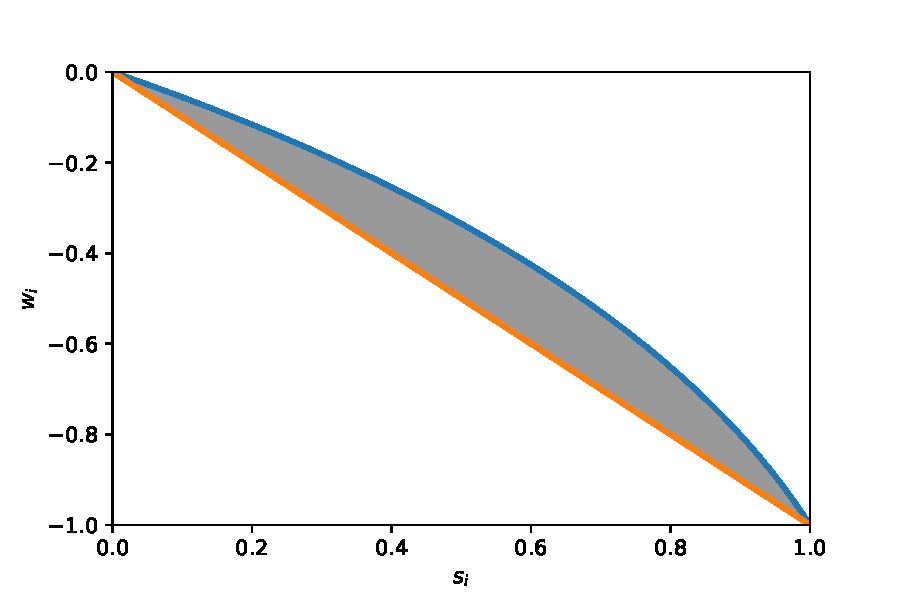
\includegraphics[scale=0.5]{codes/S-set-two-buyers.pdf}
	% 	\caption{An illustration of the set $S_i$ for $(z_i, w_i)$, which is the region bounded by (i) the line segment between $(0,0)$ and $(1,-1)$ and (ii) the arc $\Gamma_i$ (part of a quadratic curve) on the top-right of it. In this figure, we use $d_1 = 1.5$, $d_2 = 0.8$. When $d_{i+1} = d_i$, the region becomes the line segment itself.}
	% 	\label{fig:Si-illustr}
	% \end{figure}
	Let the \emph{entire} curve $\bar{\Gamma}_i$ be the extension of $\Gamma_i$ with $\alpha\in [0,1]$ replaced by $\alpha \in \mathbb{R}$.	
	It is a parabola, since it is the image of the standard parabola $\{ (\alpha, \alpha^2): \alpha\in \RR \}$ under a linear transformation given by $G_i$, i.e., $G_i \begin{bmatrix}
		\alpha \\ \alpha^2
	\end{bmatrix} = \begin{bmatrix}
		\frac{c_i}{2} \alpha^2 + d_i \alpha \\
		-\frac{c_{i+1}}{2}\alpha^2 - d_{i+1} \alpha
	\end{bmatrix}$.
	Hence, the convex hull $\conv(\bar{\Gamma}_i)$---the set of convex combinations of any finite number of points on $\bar{\Gamma}_i$---is also the image of the epigraph of the standard parabola $\mathcal{C}=\conv(\{ (\alpha, \alpha^2):\alpha\in \RR \})$ under the same linear transformation. By the convexity of $\conv(\bar{\Gamma}_i)$, we have
	$S_i = \conv(\bar{\Gamma}_i) \cap T_i$,
	where 
	$T_i = \left\{ (z_i, w_i): z_i \in [0,1],\, w_i \in [-1,0],\, z_i + w_i \geq 0 \right\}$.
	Therefore, the set $S_i$ can be represented by the linear constraints in $T_i$ and $ (z_i, w_i)\in G_i \mathcal{C}$. 
	The latter can be expanded with two additional variables $s_i, t_i$, namely, 
	$G_i \begin{bmatrix}
		s_i \\ t_i
	\end{bmatrix} = \begin{bmatrix}
		z_i \\ w_i
	\end{bmatrix},\ \begin{bmatrix}
		s_i \\ t_i
	\end{bmatrix} \in \mathcal{C}$.
	Note that the above hold for both $d_{i+1} = d_i$ and $d_{i+1} > d_i$ (if $d_{i+1} = d_i$, then $G_i$ maps the parabola $\{(t_1, t_1^2): t_1 \in \RR \}$ into the straight line $\{ (z_i, w_i): z_i + w_i = 0 \}$ and the above characterization still works).
	Substituting this and the constraints in $T_i$ into \eqref{eq:rep-U-u,z,w,a}, we obtain the desired set of constraints that characterize $u\in U(v, [0,1])$.
	Here, we do not need to include $z_i + w_i \geq 0$ in the final set of constraints: this is the same as enlarging $S_i$ to contain $(z_i, w_i)$ such that $z_i + w_i < 0$, $(z_i, w_i)\in [0,1]\times [-1, 0]$, $(z_i, w_i) \in G_i \mathcal{C}$. Doing so not affect the feasible region of $u$.

	Finally, we can also easily verify that $S_i$ is the image under linear transformation $G_i$ of the convex hull of the parabola segment $\mathcal{C}^0 = \{ (s_i, s_i^2): s_i \in [0,1] \}$, that is, 
	$\conv(\mathcal{C}^0) = \{ 0\leq s_i \leq 1,\, 0 \leq t_i \leq 1,\, s_i^2 \leq t_i \}$.
	Hence, the set of constraints (in particular, $z_i + w_i \geq 0$ and $(z_i,w_i)\in [0,1] \times [-1,0]$) imply
	$0\leq s_i, t_i \leq 1$.

	\smallskip\noindent\textbf{Proof of Theorem~\ref{thm:U-conic-rep-general-vi}}
Consider $\tilde{v}_i(\theta) = (h-l)^2 c_i \theta + (h-l)(c_i l + d_i)$, $\theta\in [0,1]$ and $\varphi(\theta) = \frac{\theta-l}{h-l}$. For any $[a,b]\subseteq [l,h]$, we have
$
	\tilde{v}_i([\varphi(a), \varphi(b)]) = \frac{(h-l)^2 c_i}{2}\left( \frac{(b-l)^2}{(h-l)^2} - \frac{(a-l)^2}{(h-l)^2} \right) + (h-l)(c_i l + d_i) \left( \frac{b-l}{h-l} - \frac{a-l}{h-l} \right) 
	= (b-a)\left( \frac{c_i}{2}(a+b) + d_i \right) = v_i([a,b])$.
Therefore, for any $u\in \RR_+^n$ such that $u_i = v_i([l_i, h_i])$ for a.e.-disjoint intervals $[l_i, u_i]\subseteq [l,u]$, we have 
$u_i = \tilde{v}_i([\varphi(l_i), \varphi(h_i)]),\, i\in [n]$
and $[\varphi(l_i), \varphi(h_i) ]\subseteq [0,1]$ are also a.e.-disjoint intervals. Let $\tilde{c}_i = (h-l)^2 c_i$ and $\tilde{d}_i = (h-l)(c_i l + d_i)$. Using Lemma~\ref{lemma:all-linear-represent-any-u}, we can easily verify that
$U(v, [l,h]) = U(\tilde{v}, [0,1])$.
%	& = \tilde{U} := 
Let $\hat{v}_i = \tilde{v}_i/\|\tilde{v}_i\|$, where $\|\tilde{v}_i\| = \tilde{v}_i([0,1]) =\frac{(l-h)^2c_i}{2} + (l-h)(c_i l + d_i) = \Lambda_i$. 
The coefficients of $\hat{v}_i$ are $\hat{c}_i$ = $\tilde{c}_i / \|\tilde{v}_i\|$ and $\hat{d}_i = \tilde{d}_i / \|\tilde{v}_i \|$, which are the same as defined in the theorem statement. Then,
$U(\tilde{v}, [0,1]) = D U(\hat{v},[0,1]) = \left\{D\hat{u}: \hat{u} \in U(\hat{v}, [0,1]) \right\}$,
where $D \in \RR^{n\times n}$ is a diagonal matrix with $D_{ii} = \|\tilde{v}_i\| = \Lambda_i$. 
Let $P\in \{0,1\}^{n\times n}$ be the permutation matrix defined in the theorem statement. Then, 
$U(\hat{v}, [0,1]) = PU(\hat{v}_\sigma, [0,1])$,
since permutation does not affect the feasibility of $x$. By Theorem~\ref{thm:U-conic-rep}, $U(\hat{v}_\sigma, [0,1])$ can be represented by $O(n)$ linear and quadratic constraints using $O(n)$ auxiliary variables.
Therefore, 
$U(v, [l,u]) = U(\tilde{v}, [0,1]) = D P U(\hat{v}_\sigma, [0,1])$
can also be represented by $O(n)$ linear and quadratic constraints using $O(n)$ auxiliary variables. 

\smallskip\noindent\textbf{Proof of Theorem~\ref{lemma:eg=>u(ik)-facts}}
First, by Lemma~\ref{lemma:U-convex-compact}, each $U_k$ is convex and compact. W.l.o.g., Assume not all $v_i$ are $0$ on $[a_{k-1}, a_k]$ (otherwise, $U_k = \{\mathbf{0}\}$ is a singleton of the $n$-dimensional zero vector, and we can remove this $k$ in all summations in the following analysis).
For any $u\in U(v, [0,1])$, there exists $x\in L^\infty([0,1])_+^n$ such that $u_i = \langle v_i, x_i\rangle$.  Let $x_{ik}$ be the restriction of $x_i$ on $[a_{k-1}, a_k]$ and $u_{ik} = \langle v_i, x_{ik}\rangle$. 
Clearly, this makes the objective value of \eqref{eq:convex-prog-u(ik)} at $(u_{ik})$ equal to that of \eqref{eq:eg-primal} at $x$. Conversely, for any $(u_{ik})$ feasible to \eqref{eq:convex-prog-u(ik)}, we can also find $x$ feasible to \eqref{eq:eg-primal} that attains the same objective value. Therefore, \eqref{eq:convex-prog-u(ik)} and \eqref{eq:eg-primal} have the same optimal objective value. 
In particular, the supremum of \eqref{eq:convex-prog-u(ik)} is attained at some $(u^*_{ik})$. 
By the Pareto optimality of $(u^*_i) \in U(v, [0,1])$ (where $u^*_i$ are the unique equilibrium utilities), an optimal solution $(u^*_{ik})$ of \eqref{eq:convex-prog-u(ik)} must satisfy $u^*_i = \sum_k u^*_{ik}$ for all $i$.

By Theorems~\ref{thm:U-conic-rep} and~\ref{thm:U-conic-rep-general-vi}, each $U_k$ can be represented by $O(n)$ variables and $O(n)$ (linear and quadratic) constraints (if some $v_i$ is zero on $[a_{k-1}, a_k]$, i.e., $v_i([a_{k-1}, a_k]) = 0$, simply remove it from the set of buyers on this interval when representing the set $U_k$). 
The set $\mathcal{C}$ is the image of an transformation of the second-order cone $\mathcal{L}$:
$(t_1, t_2) \in \mathcal{C} \ \Leftrightarrow \ t_1^2 \leq t_2 \ \Leftrightarrow \ \sqrt{\left(\frac{1-t_2}{2}\right)^2 + t_1^2} \leq \frac{1+t_2}{2} \ \Leftrightarrow \ \left( \frac{1+t_2}{2}, \frac{1-t_2}{2}, t_1 \right) \in \mathcal{L}$.
For any $u_i>0$,
	$- \log u_i = \min_{q_i\geq -\log u_i} q_i = \min_{e^{q_i} \leq u_i} (-q_i) = \min_{ (u_i, 1, q_i) \in \mathcal{E}} -q_i. \label{eq:log(ui)=>min(-qi)}$.
In this way, introducing auxiliary variables $s_i, t_i, u_i$, $i\in [n]$ the objective $\max \sum_i B_i \log \left( \sum_k u_{ik} \right)$ can be written as $-\min - \sum_i B_i q_i$, with additional (linear and exponential cone) constraints $u_i = \sum_k u_{ik}, \ 
(u_i, 1, q_i)\in \mathcal{E},\ i\in [n]$.

Combining the above analysis, we can easily reformulate \eqref{eq:convex-prog-u(ik)} into the form \eqref{eq:conic-std-form} with the said number of variables and nonzero constraint coefficients.

% % Combining the above analysis, we arrive at the overall convex conic reformulation involving only linear and (convex) conic constraints.
% % Recall that $i$ and $k$ are indices of buyers and linear segments of their valuations, respectively.

% \begin{align}
% 	\begin{split}
% 		& \min \ - \sum_i B_i q_i \ \ \st \quad \begin{rcases}
% 			   & (u_i, 1, q_i) \in \mathcal{E},\ q_i'=1, \\
% 			   & u_i = \sum_k u_{ik}, \ \ u_{\sigma^k(i) k} = \Lambda_{\sigma^k(i)k} \hat{u}_{ik}, 
% 		   \end{rcases} \quad  \forall\, i \in [n], \\[2ex]
% 		   & \begin{rcases}
% 				& \hat{u}_{1k} \leq z_{1k}, \ \ \hat{u}_{ik} \leq z_{ik} + w_{i-1,k}, \ \forall\, i=2,\dots, n-1,\ \ \hat{u}_{nk} \leq 1 + w_{nk}, \\
% 				& G_{ik}(s_{ik}, t_{ik}) = (z_{ik}, w_{ik}), \ \left(\frac{1+t_{ik}}{2}, \frac{1-t_{ik}}{2}, s_{ik}\right) \in \mathcal{L}, \\
% 				& 0\leq z_{ik} \leq 1, \ -1 \leq w_{ik} \leq 0,\ z_{ik}+w_{ik}\geq 0,\ \forall\, i \in [n],
% 			\end{rcases} \quad\forall\, k \in [K].\\[2ex]
% 	\end{split}
% 	\label{eq:overall-conic-reform} \tag{$\mathcal{CP}$}
% \end{align}
% In the above, the first group of constraints involving objective transformation, decomposition of buyers' utilities and scaling of them over subintervals.The second group represents $(\hat{u}_{1k}, \dots, \hat{u}_{nk}) \in U(\hat{v}_k, [0,1])$, where $U(\hat{v}_k, [0,1])$ is the ``standardized'' version of $U_k$ as described in Theorem~\ref{thm:U-conic-rep-general-vi}.
% To complete the proof, we calculate the number of each type of variables in the final reformulation \eqref{eq:conic-std-form}. 
% \begin{enumerate*}[(i)]
% 	\item The exponential cone variables are $(q_i, q'_i, u_i)\in \mathcal{E}$, $i\in [n]$ (with additional linear constraint $q'_i = 1$). Hence, $n_3 = O(n)$.
% 	\item For each $(s_{ik}, t_{ik})$, there is a second-order cone $\mathcal{L}$ (involving $3$ conic variables, $t_{ik}' = \frac{1+t_{ik}}{2}$, $t_{ik}'' = \frac{1-t_{ik}}{2}$ and $s_{ik}$). Hence, $n_2 = O(nK)$.
% 	\item The linear cone (nonnegative) variables are $u_{ik}$, $\hat{u}_{ik}$, $i\in [n]$, $k\in [K]$, $(z_{ik}, w'_{ik})$, $i\in [n-1]$, $k\in [K]$ ($w'_{ik} = -w'_{ik}\geq 0$) and nonnegative auxiliary variables added to transform the $O(nK)$ linear inequality constraints (in the second group of constraints in \eqref{eq:overall-conic-reform}) into equality constraints. Hence, $n_1 = O(nK)$.
% 	\item The linear equality constraints (which form ``$Ax=b$'' in the standard form \eqref{eq:conic-std-form}) are those above in \eqref{eq:overall-conic-reform} plus additional ones involving auxiliary conic variables: $q''_i = 1$, $t_{ik}' = \frac{1+t_{ik}}{2}$, $t_{ik}'' = \frac{1-t_{ik}}{2}$. Hence, $m = O(nK)$. 
% 	\item It can be easily verified that, each of the linear constraints in \eqref{eq:overall-conic-reform} (except the linear constraints $u_i = \sum_{k} u_{ik}$, $k\in[K]$), involve only a constant number of variables. 
% 	In particular, the linear equality constraints of $U_k = D^k P^k \hat{U}_k$ (i.e., last equality constraint in the first group of constraints in \eqref{eq:overall-conic-reform}) only consist of $(n)$ nonzeros, since $D^k$ and $P^k$ are diagonal and permutation matrices, respectively. 
% 	Hence, the total number of nonzeros in all linear constraints is also $O(nK)$.
% \end{enumerate*} 
% By \eqref{eq:log(ui)=>min(-qi)}, we know that the minimum $f^*$ of \eqref{eq:conic-std-form} is $-z^*$. Finally, the above reformulation does not affect feasible region of the variables $(u_i)$ and $(u_{ik})$.
% Hence, in the optimal solution of the reformulation \eqref{eq:conic-std-form}, these variables correspond to an optimal solution $(u^*_{ik})$ of \eqref{eq:convex-prog-u(ik)}.

\smallskip\noindent\textbf{Proof of Theorem~\ref{thm:ellipsoid-method-for-u(ik)-convex-program}}
We first case our problem \eqref{eq:convex-prog-u(ik)} into the standard form \cite[4.1.10]{ben2019lectures}. Same as in the paragraph below \eqref{eq:convex-prog-u(ik)}, 
let the decision variables be $(u_i)$, $(u_{ik})$, $(\hat{u}_{ik})$, $(s_{ik})$, $(t_{ik})$, $(z_{ik})$, $(w_{ik})$, with a total number of $O(nK)$. 
Here, the variables $(u_i)$, $(u_{ik})$ correspond to those in \eqref{eq:convex-prog-u(ik)}. 
The variables $(\hat{u}_{1k}, \dots, \hat{u}_{nk})$ are used to describe each ``normalized'' set of feasible utilities $\hat{U}_k$ such that $U_k = D^k P^k \hat{U}_k$.
Denote the aggregate decision variable as $x$, which has $O(nK)$ dimensions. The (minimization) objective function is 
$f(x) = - \sum_i B_i \log u_i$. 
Next, we specify the feasible region. Note that $u^*_i \in [B_i, 1]$ for all $i$ at equilibrium (the upper bound due to the normalization assumption $v_i(\Theta)=1$ and the lower bound is due to the proportionality guarantee in Theorem~\ref{thm:me-is-pareto-ef-prop}). 
Hence, we can add linear constraints $\min\{B_i, \epsilon/2\} \leq u_i \leq 1$.
without affecting the optimal solution. 
Then, ``enlarge'' the feasible sets given by the constraints by $\epsilon$ to ensure a nonempty interior of the feasible region.
\begin{enumerate*}[(i)]
	\item For each $i$, relax the equality constraint $u_i = \sum_k u_{ik}$ into $u_i \leq \sum_k u_{ik} + \epsilon$ for all $k$ (when there is no tolerance $\epsilon$, the equality constraint can clearly be relaxed to an inequality without affecting the optimum, since at optimality the inequality must be tight).
	\item For each $k$, $(u_{1k}, \dots, u_{nk})\in U_k + [0,\epsilon]^n$.
	\item For each $k$, for every linear constraint describing $U_k = D^k P^k \hat{U}_k$, that is, $u_{\sigma^k(j)k} = \Lambda_{\sigma(j) k} \hat{u}_{jk}$, relax it into $u_{\sigma^k(j)k} = \Lambda_{\sigma(j) k} \hat{u}_{jk} + \epsilon$.
	\item For each $k$, in the linear and quadratic constraints for $\hat{U}_k$, add $\epsilon$ to \emph{all} linear constraints involving $\hat{u}_{ik}$ and $z_{ik}$ or $w_{ik}$ (e.g., $\hat{u}_{ik} \leq z_{ik} + w_{i-1,k} + \epsilon$).
	\item For each $k$, relax the constraints $G_{ik} (s_{ik}, t_{ik}) = (z_{ik}, w_{ik})$ (Theorem~\ref{thm:U-conic-rep}, with the ``$k$th'' copies of the variables and the $G_i$ matrix) into $G_{ik} (s_{ik}, t_{ik}) = (z_{ik}, w_{ik}) + (\epsilon, \epsilon)$.
	\item For each $i$ and $k$, keep the constraints $0\leq z_{ik}\leq 1$, $-1\leq w_{ik}\leq 1$, $(s_{ik}, t_{ik})\in\mathcal{C}$ unchanged.
\end{enumerate*}
Constructing these constraints takes $O(nK\log n)$ time, where the $n\log n$ factor is due to sorting $\hat{d}_{1k}, \dots, \hat{d}_{nk}$ for each $k$ (see Theorem~\ref{thm:U-conic-rep-general-vi}). It is negligible compared to the running time of the ellipsoid method. 
Now, it can be easily verified that the feasible region (described by all constraints above) contains a Euclidean ball of radius $r \geq \epsilon/2$. The objective function is also convex and continuous on the feasible region. Furthermore, the total number of constraints is $O(nK)$ and each constraint only involves a constant number of variables (except $u_i = \sum_k u_{ik}$ which involves $K$ variables).

It can be easily verified that $R = \max_{x\in X} \|x\| = O(\sqrt{nK})$ since the variables $\hat{u}_{ik}$, $u_{ik}$, $u_i$ have absolute values $\leq 1+\epsilon$ (note that $\Gamma_{ik}\leq 1$) and there are $O(nK)$ variables in total. In addition, for $f^* = \min_{x\in X} f(x)$, we can see ${\rm Var}_X(f) = \max_{x\in X}f(x) - f^* \leq \log \kappa + \log \frac{2}{\epsilon}$ via simple bounds on the objective function.
Then, we can express the overall ratio $\frac{{\rm Var}_X(f) R}{\epsilon r}$ in the time complexity in \cite[4.1.2]{ben2019lectures} accordingly.
% \begin{enumerate*}[(i)]
% 	\item Each of $z_{ik}$, $w_{ik}$, $s_{ik}$, $t_{ik}$ have absolute values $\leq 1$. There are $O(nK)$ such variables. 
% 	\item The variables $\hat{u}_{ik}$ have absolute values $\leq 1+\epsilon$. There are $O(nK)$ such variables. 
% 	\item The variables $u_{ik}$ have absolute values $\leq 1+\epsilon$, since $\Lambda_{ik} = v_i([a_{k-1}, a_k]) \leq 1$. There are $O(nK)$ such variables. 
% 	\item The variables $u_i$ have absolute values $\leq 1$, as we added the constraints $\min\{B_i, \epsilon/2\} \leq u_i \leq 1$. There are $n$ such variables.
% \end{enumerate*}
% Hence, $R = O(\sqrt{nK})$.

% To bound $V$, first note that 
% $f(x) \geq -\sum_i B_i \log 1 = 0$.
% Then, since $\|B\|_1 = 1$, we have
% $f(x) \leq -\sum_i B_i \log \min\{ B_i, \epsilon/2 \} \leq \sum_i B_i \log \max\{\kappa, 2/\epsilon \} \leq \log \kappa + \log \frac{2}{\epsilon}$. 

\paragraph{The two oracles.}
The first-order oracle is trivial: the objective function is differentiable w.r.t. $u_i$ and a subgradient simply consists of the derivatives $\frac{B_i}{u_i}$. This oracle takes $T_\mathcal{G} = O(n)$ time. 
Next, we describe the separation oracle. Given a solution $x^0$ (consisting of $O(nK)$ variables in total), it clearly takes $O(nK)$ time to verify whether all constraints are satisfied. Suppose not all constraints are satisfied. There are two cases.
\begin{enumerate*}[(i)]
	\item A linear constraint is violated, say, $g^\top x^0 > a$ while $g^\top x \leq a$ for all $x\in X$. Then, this constraint itself is a separating hyperplane.
	\item A quadratic constraint is violated, say, $(s_{ik}, t_{ik}) \notin \mathcal{C} = \{(t_1, t_2): t_1^2 \leq t_2\}$. By elementary calculus, the line
	$\{ (t_1, t_2): t_2 - s_{ik}^2 = (2s_{ik}) (t_1 - s_{ik}) \}$ is tangent to the curve $\{(t_1, t_2): t_1^2 = t_2\}$ at the point $(s_{ik}, s_{ik}^2)$ on the curve. Hence, it separates $\mathcal{C}$ and $(s_{ik}, t_{ik})$.
\end{enumerate*}
Since there are $O(nK)$ linear and quadratic constraints in total, the separation oracle described above takes $T_\mathcal{S} = O(nK)$ time. 

By \cite[Theorem 4.1.2]{ben2019lectures}, the ellipsoid method finds a solution $x_\epsilon$ such that $f(x_\epsilon) - f^* \leq \epsilon$ in $N(\epsilon)$ number of calls of the oracles and $O(1)n^2N(\epsilon)$ additional arithmetic operations, where 
$N(\epsilon) = O(1) (nK)^2 \log \left( 2 + \frac{ {\rm Var}_X(f) R}{\epsilon r} \right)$.
Combining the above, the overall time complexity for computing $x_\epsilon$ is
$N(\epsilon)(T_\mathcal{S} + T_\mathcal{G}) + O(1)(nK)^2 N(\epsilon) = N(\epsilon)\left(O(n) + O(nK) + O((nK)^2) \right) \nonumber = O\left( (nK)^4 \log \frac{ \sqrt{nK}\left(\log \kappa + \log \frac{2}{\epsilon}\right) }{\epsilon} \right)  = O\left( (nK)^4 \log \frac{ nK \log \kappa }{\epsilon} \right)$. 

Here, since the feasible region has been enlarged, the minimum $f^* \leq -z^*$, where $z^*$ is the true maximum of \eqref{eq:convex-prog-u(ik)}. Therefore, $x_\epsilon$ is also $\epsilon$-close to the ``true'' minimum $-z^*$. 
Furthermore, we can transform the difference in objective value to the difference in utilities using strong convexity (where $u_i$ are part of the solution $x_\epsilon$), that is, 
	$\left(-\sum_i B_i \log u_i\right) - \left( -\sum_i B_i \log u^*_i \right) \geq \frac{\sigma}{2}\|u-u^*\|^2$, 
where a strong convexity modulus is $\sigma = \min_i B_i = \frac{1}{\kappa}$, since $u_i \leq 1$.
Therefore, for each $i$, it must hold that $|u_i - u^*_i| \leq \|u-u^*\| \leq 2\epsilon \kappa$.

To recover a fully feasible $(u_{ik})$ such that $(u_{1k}, \dots, u_{nk}) \in U_k$ and $\sum_k u_{ik} \geq u^*_i - \epsilon$, it suffices to ``discount'' $x_\epsilon$ as follows.
\begin{enumerate*}[(i)]
	\item Decrease each $\hat{u}_{ik}$ by $\epsilon$ (that is, $\hat{u}'_{ik} = \max\{ \hat{u}_{ik}-\epsilon,0 \}$), which requires each $u_{ik}$ ($i=\sigma^k(j)$) decrease by $\Lambda_{ik} \epsilon\leq \epsilon$ to ensure $u_{ik} \leq \Lambda_{ik} \hat{u}_{jk} + \epsilon$.
	\item Further decrease each $u_{ik}$ by $\epsilon$ ($u_{ik} = \max\{ u_{ik} - \epsilon, 0 \}$), which makes $u_i$ decrease by at most $(K+1) \epsilon$ to ensure $ u_i \leq \sum_k u_{ik}$.
\end{enumerate*}
We still use $(u_{ik})$ to denote the processed solution according to the above ``discounting'' procedure. This solution satisfies $(u_{1k}, \dots, u_{nk})\in U_k$ for all $k$ and $\sum_k u_{ik} \geq u_i - (K+1)\epsilon$ for all $i$. Combining this with $|u_i - u^*_i| \leq \|u-u^*\| \leq 2\epsilon \kappa$, we know that the processed solution $(u_{ik})$ approximately attains the equilibrium utilities:
$\sum_i u_{ik} \geq u^*_i - 2\kappa \epsilon - (K+1)\epsilon$.
Therefore, to ensure that $\sum_k u_{ik} \geq u^*_i - \epsilon$ for a given tolerance level $\epsilon>0$, it suffices to replace $\epsilon$ by $\frac{\epsilon}{2\kappa+ (K+1)}$, which slightly degrades the time complexity for computing $x_\epsilon$ (due to $\kappa$) and yields a said final time complexity of 
$O\left( (nK)^4 \left(\log (nK) + \log \frac{\kappa}{\epsilon}  \right) \right)$.

To construct a pure equilibrium allocation given $(u_{ik})$ is easy: since $(u_{1k}, \dots, u_{nK})\in U_k$ for each $k$, simply run Algorithm~\ref{alg:interval-partition-given-feasible-u} on $[a_{k-1}, a_k]$, where we can reuse the sorting permutations for formulating \eqref{eq:convex-prog-u(ik)}. This produces a.e.-disjoint intervals $[l_{ik}, h_{ik}]\subseteq [a_{k-1}, a_k]$ such that $v_i([l_{ik}, h_{ik}]) \geq u_{ik}$. Therefore, the pure allocation $\Theta_i := \cup_k [l_{ik}, h_{ik}]$ satisfies
$v_i(\Theta_i) \geq \sum_k u_{ik} \geq u^*_i - \epsilon$. 
